%%%%%%%%%%%%%%%%%%%%%%%%%%%%%%%%%%%%%%%%%
% Tutorial
% LaTeX Template
% Version 1.0 (09/27/17)
%
% Author:
% Ben Roose (ben.roose@wichita.edu)
%
% Original template author:
% Adam Glesser (adamglesser@gmail.com)
% www.LaTeXTemplates.com
%
% License:
% CC BY-NC-SA 3.0 (http://creativecommons.org/licenses/by-nc-sa/3.0/)
%
%%%%%%%%%%%%%%%%%%%%%%%%%%%%%%%%%%%%%%%%%

\documentclass[12pt]{article}

\usepackage{graphicx} % Allow import of images
\usepackage{subcaption} % Required for side-by-side sub figures
\graphicspath{ {images/} } % Relative path to images directory
\usepackage[margin=1in]{geometry} % Required to make the margins smaller to fit more content on each page
\usepackage[linkcolor=blue]{hyperref} % Required to create hyperlinks to questions from elsewhere in the document
\hypersetup{pdfborder={0 0 0}, colorlinks=true, urlcolor=blue} % Specify a color for hyperlinks
\usepackage{todonotes} % Required for the boxes that questions appear in
\usepackage{tocloft} % Required to give customize the table of contents to display questions
\usepackage{microtype} % Slightly tweak font spacing for aesthetics
\usepackage{palatino} % Use the Palatino font

\setlength\parindent{0pt} % Removes all indentation from paragraphs

% Create and define the list of questions
\newlistof{questions}{faq}{\large FAQ for SSH access into cslab Linux environment}
% This creates a new table of contents-like environment that will output a file with extension .faq
\setlength\cftbeforefaqtitleskip{3em} % Adjusts the vertical space between the title and subtitle
\setlength\cftafterfaqtitleskip{1em} % Adjusts the vertical space between the subtitle and the first question
\setlength\cftparskip{.3em} % Adjusts the vertical space between questions in the list of questions

% Create the command used for questions
\newcommand{\question}[1] % This is what you will use to create a new question
{
\refstepcounter{questions} % Increases the questions counter, this can be referenced anywhere with \thequestions
%\hfill
\goodbreak
\par\noindent % Creates a new unindented paragraph
\phantomsection % Needed for hyperref compatibility with the \addcontensline command
\addcontentsline{faq}{questions}{#1} % Adds the question to the list of questions
\todo[inline, color=green!40]{\textbf{#1}} % Uses the todonotes package to create a fancy box to put the question
%\vspace{0.5em} % White space after the question before the start of the answer
}

% Uncomment the line below to get rid of the trailing dots in the table of contents
%\renewcommand{\cftdot}{}

% Uncomment the two lines below to get rid of the numbers in the table of contents
%\let\Contentsline\contentsline
%\renewcommand\contentsline[3]{\Contentsline{#1}{#2}{}}

\begin{document}

%----------------------------------------------------------------------------------------
%	TITLE AND LIST OF QUESTIONS
%----------------------------------------------------------------------------------------

\begin{center}
\Huge{\bf \emph{EECS Tutorial: cslab Linux Environment SSH Access}} % Main title
\end{center}

\listofquestions % This prints the subtitle and a list of all of your questions
\bigskip % Create a gap between list and first question

\newpage % Comment this if you would like your questions and answers to start immediately after table of questions

%----------------------------------------------------------------------------------------
%	QUESTIONS AND ANSWERS
%----------------------------------------------------------------------------------------

\question{How do I access the cslab Linux environment on port 22 via an SSH client?}\label{ssh_client}

\begin{itemize}
\item The cslab-nodes are located inside a virtual private network. These internal nodes are only SSH accessible via the cslab-bastion.cs.wichita.edu jumphost. Any external connection into the cslab environment must proxy connect through the cslab-bastion and the bastion should be used only as an SSH jumphost/proxy.

\item If you are accessing cslab via SSH on WSU campus, ensure you are connected wirelessly to ``WSU Secure'' or using an Ethernet connected computer. ``WSU Guest'' wireless prohibits port 22 connections and your SSH session will fail to connect.

\item \textbf{Please only connect into the cslab environment with an SSH client if you have previous experience in using SSH and the Linux command-line. If you are new to Linux, please use the cslab \textit{Guacamole} web-browser interface.
\end{itemize}
  
\subsection*{Using \textit{PuTTY} SSH client on Microsoft Windows:}
\begin{enumerate}
%% \item You can download pre-configured \textit{PuTTY} session and host key configurations for importing into your Windows registry from this link.

  \item Download the full \textit{PuTTY} package from \href{https://www.chiark.greenend.org.uk/~sgtatham/putty/latest.html}{Simon Tatham's official download webpage} and install all \textit{PuTTY} utilities. You cannot connect to cslab with just the \textit{PuTTY} client.
  \item Run the 

  \item Open \textit{PuTTY} and in [Session] category add a new SSH connection with \break [Host Name] as \texttt{cslab-bastion.cs.wichita.edu} and [Port] as \texttt{22}.

  \item In [Connection--Data] category add your myWSU\_ID into [Auto-login username].
  \item In [Connection--SSH] category add the text \texttt{ssh cslab} into [Remote command].
  \item In [Session] category add a name for the configuration, such as ``cslab environment'' and click \textit{Save}. Saving as ``Default Settings'' will always open with this configuration.

\begin{figure}[bh!]
\centering
\begin{subfigure}{.5\textwidth}
  \centering
  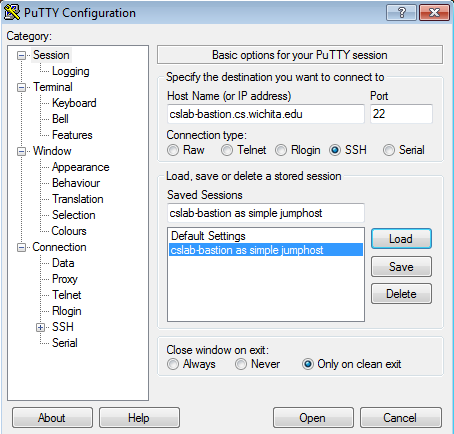
\includegraphics[width=.9\linewidth]{putty_cslab_bastion_session}
  %% \caption{A subfigure}
  \label{fig:sub1}
\end{subfigure}
\begin{subfigure}{.5\textwidth}
  \centering
  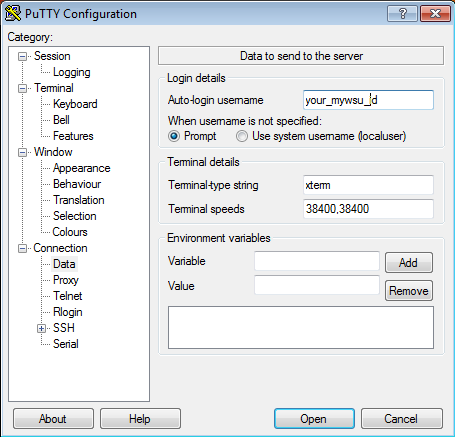
\includegraphics[width=.9\linewidth]{putty_cslab_auto_login_username}
  %% \caption{A subfigure}
  \label{fig:sub2}
\end{subfigure}%
\begin{subfigure}{.5\textwidth}
  \centering
  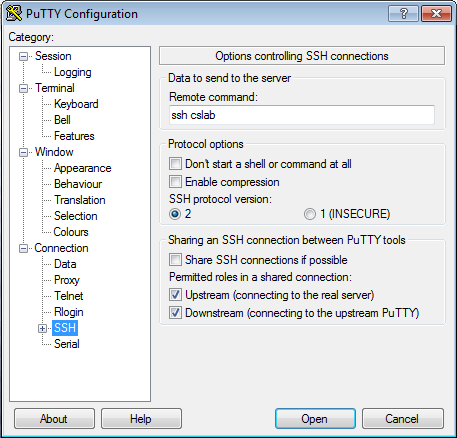
\includegraphics[width=.9\linewidth]{putty_cslab_ssh_remote_command}
  %% \caption{A subfigure}
  \label{fig:sub3}
\end{subfigure}%
\caption{\textit{PuTTY} configuration for cslab}
\label{fig:putty_config}
\end{figure}

\goodbreak
\item The first time you connect to the cslab environment using SSH, you will be asked to confirm the authenticity of each SSH remote host.
\item Ensure the cslab-bastion and cslab host key fingerprints match one of the following SHA256 or MD5 hashes before clicking \textit{Yes}:
\begin{verbatim}
ECDSA key fingerprint is
SHA256:X6dBKj4sqYYPWol6MXSQvGhpIQ6qBxh7mBQhnSw8n64
MD5:d8:ba:c6:1c:86:fa:7f:f6:92:4f:c1:02:30:ce:ab:99

ED25519 key fingerprint is
SHA256:zzozIV7cP1T9C77PLRaevzdzCu21k44lbjd8jaJKS8Q
MD5:6d:3d:8e:3a:db:f6:de:33:af:77:01:40:f3:71:1d:14

RSA key fingerprint is
SHA256:0CUyGZAYMdOd8vTOK3AtM2XTX3lMaGA2NP73rR7s6Ns
MD5:75:5a:16:53:1a:7c:c2:4b:99:66:2d:e3:1e:76:f9:c9

DSA key fingerprint is
SHA256:7zW122xr+aoBb5yiRI96nvdx8Ml07qLKHYwG2Wu6jIM
MD5:27:59:53:18:5a:67:71:f6:32:f1:e1:15:e9:e5:fe:b1
\end{verbatim}

\item You will be prompted twice to enter your myWSU password, once for the cslab-bastion (SSH jumphost/proxy) and once for the internal cslab-node.
\item You may see a \texttt{Could not chdir to home directory....} warning. Do not be concerned, this is not a critical error.
\item If the SSH connection completed successfully, then you will be presented with a standard shell prompt:

\texttt{your\_mywsu\_id@cslab-node-\#:$\sim$\$}
\end{enumerate}

\subsection*{Configuring the \textit{OpenSSH} client on Linux or Mac OSX:}
\begin{enumerate}
  \item On your Linux or Mac desktop or laptop computer, add the following host entry into your local user \texttt{ $\sim$/.ssh/config} file: \break
  (make sure to replace ``your\_mywsu\_id'' with your own 8 character ID number in both \texttt{ProxyCommand} and \texttt{User} lines.)
\end{enumerate}

\begin{verbatim}
Host cslab cslab-last cslab.cs.wichita.edu cslab-last.cs.wichita.edu
  ProxyCommand ssh your_mywsu_id@cslab-bastion.cs.wichita.edu ballast %h
  User your_mywsu_id
  IdentityFile ~/.ssh/cslab_rsa
  HostKeyAlias cslab.cs.wichita.edu
\end{verbatim}

\begin{enumerate}
  \setcounter{enumi}{1}
  \item Open a new command-line terminal emulator window.
  \item Generate a new SSH public/private key pair for your local user by typing \break
  \texttt{ssh-keygen -t rsa -b 4096}

  \item Follow the prompts in the command-line as your new SSH key is generated:
  
      \texttt{Generating public/private rsa key pair.} \break
      \texttt{Enter file in which to save the key (../id\_rsa):} Type \texttt{$\sim$\$/.ssh/cslab\_rsa} and press Enter \break
      \texttt{Enter passphrase:} Enter a passphrase you will remember! \break
      \texttt{Your identification has been saved in .../.ssh/id\_rsa.} \break
      \texttt{Your public key has been saved in .../.ssh/id\_rsa.pub.} \break
      \texttt{The key fingerprint is:} \break
      \texttt{SHA256: [fingerprint and randomart image]}
      
      \textbf{It is highly recommended to use a passphrase for your SSH key to keep your Linux user account on the cslab system secure.}
 
  \item Open the newly generated SSH public key by typing \break
  \texttt{less $\sim$\$/.ssh/cslab\_rsa.pub}
  \item Select all the text displayed within \textit{less}, starting with \texttt{ssh-rsa} and ending with the hostname of your local computer.
  \item Copy the text either by right-clicking on the terminal emulator window and selecting copy or by pressing the key combination \textbf{Ctrl+Shift+C}.
  \item Open a web-browser application and follow the ADDTUTORIALCMD to access \href{https://cslab-gateway.cs.wichita.edu/}{cslab-gateway.cs.wichita.edu}
  \item Once logged into the cslab \textit{guacamole} web-interface, open a new [cslab\_SSH\_CLI\_terminal] connection.
  \item
  \item Within the cslab SSH terminal session in your browser, open the \textit{Guacamole} menu sidebar by pressing the key combination \textbf{Ctrl+Alt+Shift}.
  \item Paste the copied text to the remote \textit{Guacamole} [Clipboard] field using your preferred method, i.e. \textbf{Ctrl+V}.
  \item Close the \textit{Guacamole} menu sidebar by pressing the key combination \textbf{Ctrl+Alt+Shift}.
  \item Within the cslab SSH terminal session, open the file \texttt{$\sim$\$/.ssh/authorized\_keys} in the \textit{nano} text editor by typing \break
  \texttt{nano $\sim$\$/.ssh/authorized\_keys}
  \item Paste your locally copied SSH public key into the terminal session by right-clicking on the browser window with your mouse or by pressing the key combination \textbf{Ctrl+Shift+V}.
  \item Make sure you have a blank line at the end of the text file by pressing \textbf{Enter} after the pasted text.
  \item Quit \textit{nano} by pressing \textbf{CTRL+X} and follow the prompts at the bottom of the screen to ensure you save the \texttt{$\sim$\$/.ssh/authorized\_keys} file.
    
  \item In a local CLI terminal connect to the cslab Linux environment by typing
\begin{verbatim}
ssh cslab
\end{verbatim}
\item The first time you connect to the cslab environment using SSH, you will be asked to confirm the authenticity of each SSH remote host, i.e.
\begin{verbatim}
The authenticity of host 'cslab.cs.wichita.edu' can't be established.
ECDSA key fingerprint is [SHA256 or MD5 hash value].
Are you sure you want to continue connecting (yes/no)?
\end{verbatim}

%\break
\item Ensure the cslab-bastion and cslab host key fingerprints match one of the following SHA256 and MD5 hashes before typing \texttt{yes}:
\begin{verbatim}
ECDSA key fingerprint is
SHA256:X6dBKj4sqYYPWol6MXSQvGhpIQ6qBxh7mBQhnSw8n64
MD5:d8:ba:c6:1c:86:fa:7f:f6:92:4f:c1:02:30:ce:ab:99

ed25519 key fingerprint is
SHA256:zzozIV7cP1T9C77PLRaevzdzCu21k44lbjd8jaJKS8Q
MD5:6d:3d:8e:3a:db:f6:de:33:af:77:01:40:f3:71:1d:14

RSA key fingerprint is
SHA256:0CUyGZAYMdOd8vTOK3AtM2XTX3lMaGA2NP73rR7s6Ns
MD5:75:5a:16:53:1a:7c:c2:4b:99:66:2d:e3:1e:76:f9:c9

DSA key fingerprint is
SHA256:7zW122xr+aoBb5yiRI96nvdx8Ml07qLKHYwG2Wu6jIM
MD5:27:59:53:18:5a:67:71:f6:32:f1:e1:15:e9:e5:fe:b1
\end{verbatim}

\item You will be prompted twice to enter your myWSU password, once for the cslab-bastion (SSH jumphost/proxy) and once for the internal cslab-node.
\item You may see a \texttt{Could not chdir to home directory....} warning. Do not be concerned, this is not a critical error.
\item If the SSH connection completed successfully, then you will be presented with a standard shell prompt:

\texttt{your\_mywsu\_id@cslab-node-\#:$\sim$\$}
\end{enumerate}

\break

%------------------------------------------------

\question{How do I use graphical (GUI) applications in cslab via an SSH client?}\label{x11_forwarding}

\textbf{Graphical applications cannot currently be accessed in Microsoft Windows using the \textit{PuTTY} SSH client. Please use the \hyperref[guac_login]{\textit{Guacamole} web-browser interface} instead. }

\subsection*{Using \textit{OpenSSH} client with X11 forwarding on Linux or Mac OSX:}
\begin{itemize}
\item Ensure you have followed the directions in \hyperref[ssh_client]{using \textit{OpenSSH} client} first.
\item SSH allows for graphical applications to run on a local computer from the remote cslab Linux environment using X11 forwarding.
\item To use X11 forwarding on a per session basis append the \texttt{-X} option flag to your SSH command, i.e.
\begin{verbatim}
ssh -X cslab
\end{verbatim}
\item To always use X11 forwarding for connections to cslab, instead of using the \texttt{-X} option flag, add the following line to the \texttt{Host cslab cslab-last....} entry in your \texttt{ $\sim$/.ssh/config} file:
\begin{verbatim}
  ForwardX11 yes
\end{verbatim}
\item If you are using Mac OSX, then you may need to install XQuartz before using X11 forwarding. Download \href{https://www.xquartz.org}{XQuartz for Mac} and install the software package.
\end{itemize} 

%------------------------------------------------

\question{How do I copy files from/to the cslab Linux environment via an SSH client?}\label{scp_copying}

\subsection*{Using \textit{OpenSSH} client on Linux or Mac OSX:}
\begin{itemize}
\item Ensure you have followed the directions in \hyperref[ssh_client]{using \textit{OpenSSH} client} first.
\item To copy a file from your local computer to your user home directory on cslab using Secure Copy (SCP), type

\texttt{scp local\_filename\_or\_path cslab:$\sim$}

\item To copy a file from your user home directory on cslab to a local directory on your local computer, type

\texttt{scp cslab:$\sim$/remote\_filename\_or\_path local\_directory}
\end{itemize}

%------------------------------------------------

\question{How do I access the last accessed cslab-node via an SSH client?}\label{ssh -last}

\begin{itemize}
\item When connecting to the cslab Linux environment using an SSH client, the ballast load-balancer on cslab-bastion will redirect you to one of the available and least used cslab-nodes at time of connection. Since load-balancing is calculated by ballast on a one minute cycle, you may not be redirected to the same cslab-node the next time you connect into cslab using SSH.

\item \textbf{Use the following instructions to connect to the last used cslab-node only if/when you need access into a previously running SSH connection. For normal use, your best option is always to connect via \texttt{ssh cslab} and let the ballast load-balancer automatically connect to an available node.}
\end{itemize}

\subsection*{Using \textit{OpenSSH} client on Linux or Mac OSX:}
\begin{enumerate}
\item If you need to connect to the last cslab-node you previously accessed using SSH, just append \texttt{-last} to the SSH command, i.e.
\begin{verbatim}
ssh cslab-last
\end{verbatim}
\end{enumerate}

\subsection*{Using \textit{PuTTY} SSH client on Microsoft Windows:}
\begin{enumerate}
\item Open \textit{PuTTY} and load the previously created ``cslab environment'' session.
\item Change [Connections--Data] configuration category [Remote command] entry to \texttt{ssh cslab-last}.
\item \textit{Save} changed configuration as a new [Session] with a different name, such as ``cslab environment last used node''.
\item If you need to connect to the last cslab-node you previously accessed using SSH, connect using this newly created \textit{PuTTY} session.
\end{enumerate}

%------------------------------------------------
\break
\question{What are the currently known bugs/glitches within the cslab Linux environment?}\label{known_bugs}

Due to the cslab environment being so new, there are a few software bugs and glitches which you may see at times. Most of these bugs occur during operations that involve the new cslab environment interacting with the older CS servers and functions and are not critical issues.

Known bugs include:
\begin{itemize}
  \item A policykit error message pops up when user first logs into a \textit{Guacamole} RDP desktop session if other users are also logged in. This is a minor bug within policykit and can be easily mitigated by clicking \textit{Okay} in the pop-up window.
  \item When the \textit{handin} command is used in the cslab environment for programming assignment submission it may produce a \texttt{segmentation fault} error. This is caused by the older 32-bit \textit{handin} program running on the cslab 64-bit processor architecture. The error is minor and does not affect submission of student assignments for grading.
  %% \item When accessing cslab via an SSH client through the cslab-bastion, a \texttt{Could not chdir to home directory....} warning may be displayed. This is caused by cslab-bastion not having access to user home directories as an SSH connection is established. cslab-bastion is only used as an SSH jumphost to allow for external access into the cslab-nodes, and does not require access to user home directories for this function. The warning can be disregarded.
%%   \item Graphical (GUI) applications cannot currently be accessed in Microsoft Windows using the \textit{PuTTY} SSH client. This is due to a limitation with the \textit{PuTTY} client which requires SSH public key authentication for using the cslab-bastion as a secure SSH proxy. Adding public key authentication for SSH access into cslab is planned as a future option. For now, please use the \hyperref[guac_login]{\textit{Guacamole} web-browser interface} when graphical applications are required from a Microsoft Windows computer.
\end{itemize}

\textbf{If you experience a bug or error when using the cslab Linux environment which stops you from completing your programming assignments, please inform your instructor at your earliest convenience.}


%------------------------------------------------

\end{document}
